\section{Алгоритм формирования пары <<образ "--- значение>> нового знака} \label{sect3_3}

\subsection{Общая схема образования знака}

В соответствии с тем, что было сказано при описании синтаксического уровня модели картины мира в главе \ref{chapt2}, до того, как происходит связывание компонент знака в единую структуру под одним именем, существуют лишь <<парные>> переходы между компонентами знания агента о том или ином явлении. До моментам именования эти компоненты образуют <<протознак>>:
\begin{itemize}
	\item перцепт становится образом знака после выполнения процедуры именования,
	\item функциональное значение "--- значением знака,
	\item биологический смысл "--- личностным смыслом знака.
	\end{itemize}
	
С введением этой структуры схема алгоритма формирования нового знака будет иметь следующий вид \cite{PanovA2014a}.

\begin{enumerate}
	\label{new_sign_alg}
	\renewcommand\labelenumi{\theenumi .}
	\item\label{stage1} Формирование перцепта.
	\item\label{stage2} Порождение на основе прошлого опыта или на основе прецедентов "--- множества пар вида <<перцепт "--- функциональное значение>> "--- функционального значения объекта.
	\item\label{stage3} Получение субъектом из культурной среды, аккумулированной в системе естественного языка, пары <<имя знака "--- значение>> и оценка специальным механизмом степени близости функционального значения, построенного на стадии \ref{stage1} к значению, полученному из культурной среды; в случае недостаточной близости "--- переход к стадии \ref{stage1} и продолжение формирования перцепта.
	\item\label{stage4} Связывание имени из пары <<имя знака "--- значение>> с перцептом, построенным после завершения выполнения стадий \ref{stage1}--\ref{stage3}; с этого момента перцепт превращается в образ.
	\item Формирование личностных смыслов знака на основе прецедентов действий с предметом.
	\item Связывание имени из пары <<имя знака "--- значение>> со сформированным личностным смыслом. С этого момента функциональное значение превращается в значение, а биологический смысл "--- в личностный смысл.
	\item Продолжение отображения <<биологический смысл "--- перцепт>> включением в область определения отображения личностного смысла, полученного в предыдущем пункте, а в область значений отображения "--- образа из стадии \ref{stage4}.
\end{enumerate}

Наиболее существенным моментом в приведённом алгоритме является итерационный процесс на стадиях \ref{stage1}--\ref{stage3}. Данный параграф будет посвящён исследованию этого процесса.

\subsection{Процедурные и объектные признаки}

Введём семейство бинарных отношений $\{\sqsubset,\sqsubset^1,\sqsubset^2,\dots\}$, определённых на декартовом произведении $\mathcal F\times \mathcal F$. Будем считать, что признак $f_1$ поглощается признаком $f_2$, $(f_1,f_2 )\in\sqsubset$ или $f_1\sqsubset f_2$, в том случае, если $f_1\dashv R_1^j, f_2\dashv R_2^{j+1}$, $R_2^{j+1}$ "--- родительский $R$-автомат по отношению к $R_1^j$ и в множестве матриц предсказания $\mathcal Z_2$ признака $f_2$ существует как минимум одна матрица $Z_r^2$, содержащая некоторый столбец $\bar z_u^r$ с элементом $z_{uv}^r\not=0$, где $v$ "--- индекс признака $f_1$ во входном векторе для распознающего автомата $R_2^{j+1}$ (Рисунок \ref{fig:rb_measure}).

\begin{figure}[h]
	\centering
	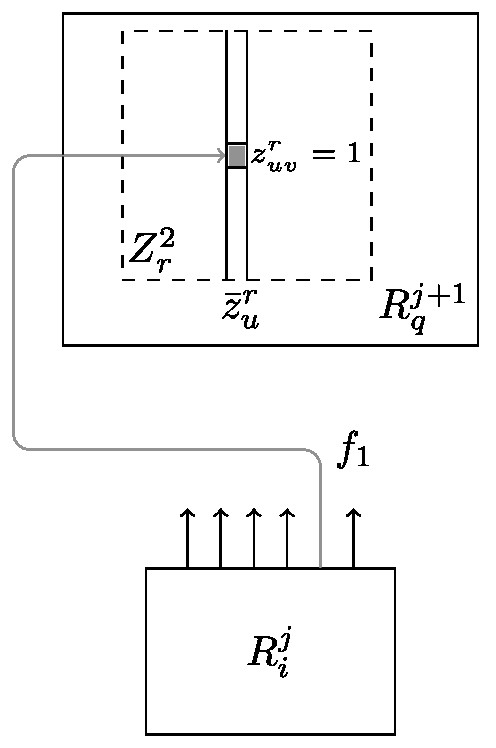
\includegraphics[width=0.3\linewidth]{automata/meas}
	\caption{Определение отношения поглощения на множестве признаков.}
	\label{fig:rb_measure}
\end{figure}

Пара признаков $(f_1,f_2)\in\sqsubset^t$ или $f_1\sqsubset^t f_2$, где $t\in\{1,2,\dots\}$, в~том случае, если $f_1\dashv R_1^j, f_2\dashv R_2^{j+1}$, $R_2^{j+1}$ "--- родительский $R$-автомат по отношению к $R_1^j$ и в множестве матриц предсказания $\mathcal Z_2$ признака $f_2$ существует как минимум одна матрица $Z_r^2$, содержащая $t$–ый столбец $\bar z_t^r$ с~элементом $z_{tv}^r\not=0$, где $v$ "--- индекс признака $f_1$ во~входном векторе для распознающего автомата $R_2^{j+1}$.

Каждый элемент векторов"--~столбцов соотносится с признаком из входного множества признаков распознающего автомата, что означает задание индекса для каждого входного признака. Индекс признака $f_k\in\mathcal F_i^j$ равен $q$, если ему соответствует $q$-ый элемент векторов"--~столбцов матриц предсказания распознающего автомата $R_i^j$. 

Введём операцию $\Lambda$, которая по множеству матриц распознавания $\mathcal Z_k$ признака $f_k$ определяет два набора индексов столбцов матриц из $Z_k$. Первый набор $I_c=\{i_1^c,i_2^c,\dots\}$, $\forall k\ 0\leqslant i_k^c < h$, составляют индексы \textit{столбцов условий}, в которых ненулевые элементы определяют условия проявления признака $f_k$. Второй набор $I_e=\{i_1^e,i_2^e,\dots\}$, $\forall k\ 0\leqslant i_k^e < h$, состоит из индексов  \textit{столбцов эффектов}, в которых ненулевые элементы определяют эффекты проявления признака $f_k$. Примером реализации процедуры $\Lambda$ может служить алгоритм Норриса по поиску максимального прямоугольного подмножества в бинарном отношении \cite{Norris1977}.

\begin{Def}
	Признаки, для матриц предсказания которых процедура $\Lambda$ выдаёт не пустые множества индексов $I_c$ и $I_e$, будем называть процедурными признаками, остальные "--- объектными признаками.
\end{Def}

Введение данного определения означает, что всё множество признаков делится на два подмножества: $\mathcal F=\mathcal F^{proc}\cup\mathcal F^{obj}$ и $\mathcal F^{proc}\cap\mathcal F^{obj}=\varnothing$.

Для любого процедурного признака выполняются следующие естественные условия:
\begin{itemize}
	\item условие всегда предшествует эффекту,
	\item условие всегда влечёт за собой эффект и
	\item все условия всегда отделены от своих эффектов.
\end{itemize}

Иными словами, если $f_1$ "--- процедурный признак, то если столбец $\bar z_u^r$ матрицы предсказания $Z_r^1$ является столбцом условий, т.~е. $u\in{I_c}$, этот столбец не может одновременно являться столбцом эффектов, т.~е. $u\not\in I_e$, и существует такое $t>0$, что столбец $\bar z_{u+t}^r$ является столбцом эффектов, т.~е. $u+t\in I_e$.

Пополним семейство отношений $\{\sqsubset,\sqsubset^1,\sqsubset^2,\dots\}$ двумя отношениями: $\sqsubset^c$ и $\sqsubset^e$, принадлежность к~которым пары признаков $(f_1,f_2)$ свидетельствует о~том, что признак $f_1$ присутствует соответственно в~столбце условий и эффектов как минимум в~одной матрице предсказания процедурного признака $f_2$.

\subsection{Определение компонент знака}

При образовании нового знака $s$ до того, как формируемая тройка компонент, называемая протознаком, получит имя, будем считать,~что будущему знаку $s$ \textit{соответствует} некоторый признак $f\in\mathcal F$, обладающий перцептом, функциональным значением и биологическим смыслом, которые после завершения процесса формирования знака становятся, соответственно, образом, значением и личностным смыслом.
\begin{Def}
	Если $f_1$ "--- признак, соответствующий знаку $s_1$, то подмножество $\tilde p(f_1)\subseteq\mathcal F$ таких признаков, что $\forall f_i\in\tilde p(f_1) f_i\sqsubset f_1$, будем называть перцептом признака $f_1$ (образом знака $s_1$).
\end{Def}

На множестве всех перцептов $\tilde P$ введём величину $\rho_p(\tilde p(f_1),\tilde p(f_2))$, вычисляемую по~следующему правилу:
\begin{itemize}
	\item если $f_1$ и $f_2$ распознаются разными распознающими автоматами, т.~е. $f_1\dashv R_1^j, f_2\dashv R_2^i$, то $\rho_p(\tilde p(f_1),\tilde p(f_2))=\infty$,
	\item если $f_1$ и $f_2$ распознаются одним и тем~же распознающим автоматами $R_1^j$ со~множеством входных признаков $F_1^j$ мощности $q$ и характерным временем $h$, то
	\begin{equation}
		\rho_p(\tilde p(f_1),\tilde p(f_2))=\min\limits_{\substack{Z_r^1\in Z_1\\Z_s^2\in Z_2}}\frac{1}{q\cdot h}\sum\limits_{u=1}^h\|\bar z_u^r-\bar z_u^s\|.
	\end{equation} 
\end{itemize}

\begin{Pred}
	Величина $\rho_p$ является метрикой на множестве перцептов $\tilde P$.
\end{Pred}

\begin{Proof}
	Свойства тождества и симметрии очевидны вследствие свойств введённой нормы. Проверим неравенство треугольника. В том случае, когда признаки,~распознаются разными автоматами "--- неравенство следует из свойств бесконечности. Во втором случае, в следствие того, что $q$ и $h$ являются константами, то неравенство следует из неравенства треугольника для введённой нормы.
\end{Proof}

\begin{Def}
	Если $f_1$ "--- признак, соответствующий знаку $s_1$, $f_2$ "--- процедурный признак, $f_1\sqsubset^c f_2$, то будем называть $f_2$ элементом функционального значения признака $f_1$ (элементом значения знака $s_1$). Множество всех элементов функционального значения признака $f_1$ будем обозначать $\tilde m(f_1)$.
\end{Def}

На множестве всех функциональных значений $\tilde M$ введём величину $\rho_m(\tilde m(f_1),\tilde m(f_2))$, вычисляемую по следующему правилу:
\begin{equation}
	\rho_m(\tilde m_1(f_1),\tilde m_2(f_2 ))=\min\limits_{\substack{f_i\in\tilde m(f_1 )\\f_j\in\tilde m(f_2 )}}\rho_p(\tilde p(f_i ),\tilde p(f_j )).
\end{equation}

\begin{Pred}
	Величина $\rho_m$ является метрикой на множестве функциональных значений $\tilde M$.
\end{Pred}

\begin{Proof}
	Очевидно вследствие того, что функция $\rho_p$ является метрикой, а функция минимума не меняет свойств метрики.
\end{Proof}

\subsection{Семантический уровень обобщения} 

На основе описанной модели компонент знака становится возможным описать процедуры обобщения (см. первую часть работы) на модельном, семантическом уровне. Для этого будем считать, что матрицы предсказания распознающих автоматов были сформированы в процессе обучения (например, с использованием алгоритма HTM \cite{Hawkins2009} или THSOM \cite{Koutn2008}). При рассмотрении множества матриц предсказания $\mathcal Z$ некоторого распознающего автомата возникают следующие три основных случая:

\begin{itemize}
	\item \textit{Внутреннее обобщение}. Будем называть схожими, такие матрицы из подмножества $Z'_k=\{Z_1^k,Z_2^k\dots,Z_m^k\}$ множества матриц предсказания $Z_k$ некоторого признака $f_k$, для которых при $\forall i,j,l$ таких, что $Z_i,Z_j\in Z'_k,l\in\{0,\dots,h\}$ выполняется $card(z_l^i\wedge z_l^j)<c_3$, где $c_3$ "--- некоторая константа. Обобщение в этом случае заключается в замене подмножества схожих матриц $Z'_k$ одной обобщённой $Z^*=(\bigwedge\limits_{Z_q\in Z'_k}\bar z_1^q,\bigwedge\limits_{Z_q\in Z'_k}\bar z_2^q,\dots,\bigwedge\limits_{Z_q\in Z'_k}\bar z_h^q)$. Таким образом, осуществляется кластеризация множества матриц предсказания признака $f_k$, контролируемая одним параметром близости $c_3$.
	\item \textit{Конкретизация}. В~тех случаях, когда получаемые с использованием описанной выше меры близости кластеры матриц предсказания признака $f_k$ расходятся достаточно сильно, образуются новые конкретизированные признаки для каждого кластера и соответственно расширяется множество выходных признаков $F^*$ распознающего автомата.
	\item \textit{Внешнее обобщение}. В~том случае когда во~всех матрицах предсказания $R$-автоматов, являющихся родительскими по отношению к распознающему автомату $R$, $i$-ые и $j$-ые компоненты всех столбцов матриц принимают одинаковые значения, выходные признаки $f_i,f_j\in F^*$, соответствующие этим компонентам, обобщаются в один признак с объединённым множеством матриц предсказания. При этом возможно и дальнейшее внутреннее обобщение.
\end{itemize}

Отдельно необходимо рассмотреть случай \textit{абстрагирования}, когда несколько выходных признаков одного или нескольких распознающих автоматов в результате работы процедуры обобщения на синтаксическом уровне (см. первую часть работы) формируют новый признак $f^*$ в некотором $R$-автомате $R^*$, лежащем на следующем уровне иерархии. В этом случае матрица предсказания будет состоять из единственного столбца с ненулевыми элементами, которые соответствуют признакам, составляющим данную категорию.

И, наконец, ещё один случай обобщения на семантическом уровне заключается в образовании ролевой структуры процедурных признаков. Рассмотрим случай, когда столбцы условий или эффектов некоторых матриц предсказания процедурного признака $f_p$ различаются только в двух компонентах, т.~.е. $i$-ая компонента в некоторых столбцах равна $1$, а в других "--- $0$, а $j$-ая компонента наоборот "--- в первых равна $0$, а во вторых "--- $1$. Если соответствующие этим компонентам признаки в результате абстрагирования попали в некоторую общую категорию $f_{cat}$, то к множеству матриц предсказания признака $f_p$ добавляется матрица с новой компонентой, соответствующей признаку $f_{cat}$ и обнулёнными компонентами $i$ и $j$. Данная процедура легко распространяется на случай, когда количество элементов категории $f_{cat}$ в матрицах предсказания признака $f_p$ больше двух. Таким образом, для процедурного признака $f_p$ появляется обобщённая, ролевая матрица предсказания.

\subsection{Свойства на множестве признаков}

В целях дальнейшего изложения рассмотрим подробнее строение матрицы предсказания процедурного признака. Матрицу предсказания $Z_r^p$ процедурного признака $f_p$ всегда можно представить в следующем виде:
\begin{equation}
Z_r^p=(\bar z_1^{r,c},\dots,\bar z_{j_1}^{r,c},\bar z_{j_{1+1}}^{r,e},\dots,\bar z_{i_1}^{r,e},\dots,\dots,\bar z_{i_{k-1}+1}^{r,c},\dots,\bar z_{j_k}^{r,c},\bar z_{j_k+1}^{r,e},\dots,\bar z_{i_k}^{r,e}),
\end{equation}
где $\bar z_j^{r,c}$ "--- столбцы причин, $\bar z_i^{r,e}$ "--- столбцы следствий. 

Величину $k$ будем называть \textit{сложностью} процедурного признака. В~дальнейшем будем рассматривать простые матрицы предсказаний $k$-сложного процедурного признака:
\begin{equation}
Z_r^p=(\bar z_1^{r,c},\bar z_2^{r,e},\dots,\dots,\bar z_{2\cdot k-1}^{r,c},\bar z_{2\cdot k}^{r,e}).
\end{equation}
Краткая форма $k$-сложного процедурного признака $f_p$ имеет матрицу предсказания, в которой оставлены только первый столбец условий и последний столбец эффектов.

Любой односложный, или элементарный, процедурный признак $f_p$, распознаваемый автоматом $R_i^j$, можно представить в виде правила $r_p=(F_C(f_p),F_A(f_p),F_D(f_p))$, в котором:
\begin{itemize}
	\item $F_C (f_p )\subseteq F_i^j$ "--- множество признаков "--- условий правила: $\forall f\in F_C(f_p)$ $f\sqsubset^c f_p$;
	\item $F_A(f_p)\subseteq F_i^j$ "--- множество добавляемых правилом признаков: $\forall f\in F_A(f_p)$ $f\sqsubset^e f_p,f\notin F_C$;
	\item $F_D(f_p)\subseteq F_i^j$ "--- множество удаляемых правилом признаков: $\forall f\in F_D(f_p)$ $f\notin F_A,f\in F_C$.
\end{itemize}

Очевидно, выполняются следующие соотношения: $F_A(f_p)\cap F_D(f_p)=\varnothing, F_A(f_p)\cap F_C(f_p)=\varnothing, F_D(f_p)\subseteq F_C(f_p)$.

\begin{Def}
	Процедурный признак $f_p^1$ c матрицей предсказания $Z=(\bar z_1^c,\bar z_2^e)$ выполняется на векторе $z$ длины $q$, если $z\cdot \bar z_1^c=\bar z_1^c$.
\end{Def}
Будем говорить, что процедурный признак $f_p^1$ выполним в~условиях процедурного признака $f_p^2$, если 
\begin{itemize}
	\item оба признака распознаются одним и тем~же распознающим автоматом $R_i^j$ и признак  $f_p^1$ выполняется на~столбце условий матрицы предсказания признака $f_p^2$,
	\item $f_p^1\dashv R_1^{j_1}, f_p^2\dashv R_2^{j_2}$, множества $F_C(f_p^1 )$ и $F_C(f_p^2)$ состоят из~одних и тех~же признаков, образуемый вектор $\tilde z$ (той же мощности, что и множество $F_1^{j_1}$) элементы которого, соответствующие признакам из $F_C(f_p^2)$ принимаются равными $1$,  остальные "--- $0$, и признак $f_p^1$ выполним на~векторе $\tilde z$. 
\end{itemize}

\begin{Def}
	Будем говорить, что два процедурных признака $f_p^1$ и $f_p^2$ конфликтуют, если выполнено как минимум одно из~следующих условий:
	\begin{itemize}
		\item $F_D(f_p^1)\cap F_A(f_p^2)\not=\varnothing$,
		\item $F_D(f_p^2)\cap F_A(f_p^1)\not=\varnothing$,
		\item $F_D(f_p^1)\cap F_C(f_p^2)\not=\varnothing$,
		\item $F_D(f_p^2)\cap F_C(f_p^1)\not=\varnothing$.
	\end{itemize}
\end{Def}

\begin{Def}
	Результатом операции сохраняющего приведения вектор"--~столбца $\bar z_1$ к~множеству входных признаков $F_{i_2}^{j_2}$ будем называть такой вектор $\bar z_3$ длины $q_{i_2}^{j_2}$, элемент которого $z_{3k}=1$, если $f_{i_1}^{j_1}(k)=f_{i_2}^{j_2}(k)$ и $z_{1k}=1$, иначе $z_{3k}=0$, и обозначать $(\bar z_1\rightarrow F_{i_2}^{j_2})=\bar z_3$.
\end{Def}

\begin{Def}
	Результатом операции сужающего приведения вектор"--~столбца $\bar z_1$ к~некоторому столбцу $\bar z_2$ распознающего автомата $R_{i_2}^{j_2}$ будем называть такой вектор $\bar z_3$ длины $q_{i_2}^{j_2}$, элемент которого $z_{3k}=1$, если $f_{i_1}^{j_1}(k)=f_{i_2}^{j_2}(k)$, $z_{2k}=1$ и $z_{1k}=1$, иначе $z_{3k}=0$, и обозначать $(\bar z_1\Rightarrow \bar z_2)=\bar z_3$.
\end{Def}

\subsection{Опыт наблюдения и алгоритм $\mathfrak A_{pm}$}

Будем считать, что у субъекта имеется опыт наблюдения, который выражается в виде отношения $\Psi_p^m: \Psi_p^m(\tilde p)=\tilde m$, в том случае, если $\tilde p\in\tilde P$ является перцептом некоторого признака $f$, а $\tilde m\in\tilde M$ "--- функциональным значением того же признака $f$.

На странице \pageref{alg:cycle_pm} представлен алгоритм доопределения функции $\Psi_p^m$, который и представляет собой суть итерационного процесса во время образования знака согласно алгоритму на странице \pageref{new_sign_alg}. Доопределение проводится на~новую пару $(\tilde p,\tilde m)$, где функциональное значение $\tilde m$ строится в сравнении с эталоном $\tilde m^0$, а перцепт $\tilde p$ формируется на основе подмножества составляющих признаков $\hat F$. Доопределение функции $\Psi_p^m$ означает формирование нового признака $f^*$, т.~е. его первой матрицы предсказания $Z^*$ в~рамках распознающего автомата $R^*$.

\begin{algorithm}[H]
	\caption{Алгоритм $\mathfrak{A}_{pm}$}
	\label{alg:cycle_pm}
	\begin{algorithmic}[1]
			\Require $\tilde m^0=\{f_p\}, \Psi_p^m, \hat F\subseteq \mathcal F$;
	
	\State $\tilde p^{*(0)} := \varnothing$;
	\State $Z^{*(0)} := \varnothing$;
	\State $t := 0$;
	
	\ForAll{$f^{(t)}\in \hat F$}
		\If{$\exists \tilde m^{(t)}\in \tilde M$ такое, что $(\tilde p(f^{(t)}),\tilde m^{(t)})\in\Psi_p^m$, $\tilde m^{(t)}$ выполним в условиях признака $f_p$, $\nexists f: f\in\tilde p^{*(t)},(\tilde p(f),\tilde m(f))\in\Psi_p^m, \tilde m^0$ конфликтует с $\tilde m^{(t)}$}
			\State $\tilde p^{*(t)}=\tilde p^{*(t)}\cup\{f^{(t)}\}$;
	
			\If{$\exists R_i^j$ такой, что $f^{(t)}\in F_i^j$}
				\State $R_i^{j(t)}:=R_i^j$;
			\Else
				\State $R_i^{j(t)}:=\argmax\limits_{\mathcal R} (F_i^j\cap\tilde p^{(t)}), F_i^{j(t)}:=F_i^{j(t)}\cup f^{(t)}$;
			\EndIf
	
			\State $\bar z_s:=(z_{s1},z_{s2},\dots,z_{sq}), z_{sk}=1$, если $k$ -- индекс признака $f^{(t)}$ во входном векторе распознающего блока $R_i^{j(t)}$ и $z_{sk}=0$ иначе;
			\State $Z^{*(t)}:=Z^{*(t)}\cup\bar z_s$;
			\State $Z_p^{(t)}:=(\bar z_1^{c(t)},\bar z_2^{e(t)},\dots,\bar z_{2\cdot k-1}^{c(t)},\bar z_{2\cdot k}^{e(t)})$, где $\bar z_i^{c(t)}=\bigvee\limits_{\tilde m_j^{(t)}}(\bar z_j^{c(t)}\rightarrow F_p^j),$ 
	\\\hspace{3.0cm}$\bar z_i^{e(t)}=\bigvee\limits_{\tilde m_j^{(t)}}(\bar z_j^{e(t)}\Rightarrow\bar z_j^e)$;
		\EndIf
	
		\State $\tilde m^{*(t)}=\{f_p^{(t)}\}$;
		\State $\mathcal Z^{*(t)}=\{Z^{*(t)}\}$;
		\State $t=t+1$;
	\EndFor
	
	\Return $\Psi_p^m$, определённая на паре $(\tilde p, \tilde m)$, где $\tilde p=\tilde p^{*(|\hat F|)}$, $\tilde m=\tilde m^{*(|\hat F|)}$, $f^*, Z^*=Z^{*(|\hat F|)},\mathcal Z^*=\{Z^*\}$;
	\end{algorithmic}
\end{algorithm}

Для обоснования данного алгоритма необходимо доказать сходимость функциональных значений, которые строятся в процессе его выполнения, к эталонному значению $\tilde m^0$.

%============================================================================================================================

\subsection{Корректность алгоритма $\mathfrak A_{pm}$} \label{sect3_4}

\begin{Theorem}[о корректности алгоритма $\mathfrak A_{pm}$]
	Алгоритм $\mathfrak A_{pm}$ корректен, т.~е. последовательность функциональных значений $\langle\tilde m^{*(0)},\tilde m^{*(1)},\dots\rangle$, которая строится с помощью алгоритма $\mathfrak A_{pm}$ для функционального значения $\tilde m^0$, стремится к $\tilde m^0$.
\end{Theorem}

\begin{Proof}
	Рассмотрим два элемента последовательности $\tilde m^{*(t)}=\{f_p^{(t)}\}$ и $\tilde m^{*(t+1)}=\{f_p^{(t+1)}\}$. Соответствующие матрицы предсказания будут иметь следующий вид:
	\begin{eqnarray}
		Z_p^{(t)}=(\bar z_1^{c(t)},\bar z_2^{e(t)},\dots,\dots,\bar z_{2\cdot k-1}^{c(t)},\bar z_{2\cdot k}^{e(t)}),\\
		Z_p^{(t+1)}=(\bar z_1^{c(t+1)},\bar z_2^{e(t+1)},\dots,\dots,\bar z_{2\cdot k-1}^{c(t+1)},\bar z_{2\cdot k}^{e(t+1)}).
	\end{eqnarray}
	Если на шаге 1 и 2 алгоритма $\mathfrak A_{pm}$ на $(t+1)$-й итерации не был найден подходящий признак, то матрицы $Z_p^{(t)}$ и $Z_p^{(t+1)}$ равны. Рассмотрим случай, когда был найден подходящий признак $f^{(t+1)}$ с функциональным значением $\tilde m^{(t+1)}=\{\tilde f_p^{(t+1)}\}$ с соответствующей матрицей предсказания $\tilde Z_p^{(t+1)}=(\bar z^{c(t+1)},\bar z^{e(t+1)})$.
	
	Т.~к. выполнено условие шага 1, то признак $\tilde f_p^{(t+1)}$ выполним на некотором $(2\cdot s-1$-м столбце условий матрицы предсказания признака $f_p$. Это означает, что матрицы $Z_p^{(t)}$ и $Z_p^{(t+1)}$ будут отличать только в двух вектор-столбцах $(2\cdot s-1)$-м и $(2\cdot s)$-м:
	\begin{equation}
		\bar z_{2\cdot s-1}^{c(t+1)}=\bar z_{2\cdot s-1}^{c(t)}\vee (\bar z^{c(t+1)}\rightarrow F_p^j),\bar z_{2\cdot s}^{e(t+1)}=\bar z_{2\cdot s}^{e(t)}\vee(\bar z^{e(t+1)}\Rightarrow \bar z_{2\cdot s}^e).
	\end{equation}
	По определению расстояние между функциональными значениями $\tilde m^{(t)}$ и $\tilde m^0$ примет следующее значение:
	\begin{eqnarray}
		\rho_m(\tilde m^{(t)},\tilde m^0)=\min\limits_{\substack{f_i\in\tilde m^{(t)}\\f_j\in\tilde m^0}}\rho_p(\tilde p(f_i),\tilde p(f_j ))=\rho_p(\tilde p(f_p^{(t)}),\tilde p(f_p))=\nonumber \\
		=\frac{1}{q\cdot h}\sum\limits_{\substack{\bar z_u^1\in Z_p^{(t)}\\\bar z_u^2\in Z_p}}\|\bar z_u^1-\bar z_u^2\|.
	\end{eqnarray}
	Аналогично для $\tilde m^{(t+1)}$:
	\begin{equation}
		\rho_m(\tilde m^{(t+1)},\tilde m^0)=\frac{1}{q\cdot h}\sum_{\substack{\bar z_u^1\in Z_p^{(t+1)}\\\bar z_u^2\in Z_p}}\|\bar z_u^1-\bar z_u^2\|.
	\end{equation}
	Рассмотрим разность 
	\begin{eqnarray}
		\rho_m(\tilde m^{(t)},\tilde m^0)-\rho_m(\tilde m^{(t+1)},\tilde m^0)=\frac{1}{q\cdot h}(\|\bar z_{2\cdot s-1}^{c(t)}-\bar z_{2\cdot s-1}^c\|+\|\bar z_{2\cdot s}^{e(t)}-\bar z_{2\cdot s}^e\|-\nonumber \\
		-\|\bar z_{2\cdot s-1}^{c(t+1)}-\bar z_{2\cdot s-1}^c\|-\|\bar z_{2\cdot s}^{e(t+1)}-\bar z_{2\cdot s}^e\|)=\frac{1}{q\cdot h}(\|\bar z_{2\cdot s-1}^{c(t)}-\bar z_{2\cdot s-1}^c\|+\nonumber \\
		+\|\bar z_{2\cdot s}^{e(t)}-\bar z_{2\cdot s}^e\|-\|\bar z_{2\cdot s-1}^{c(t)}\vee(\bar z^{c(t+1)}\rightarrow F_p^j)-\bar z_{2\cdot s-1}^c\|-\nonumber \\
		-\|\bar z_{2\cdot s}^{e(t)}\vee(\bar z^{e(t+1)}\Rightarrow\bar z_{2\cdot s}^e)-\bar z_{2\cdot s}^e\|),
	\end{eqnarray}
	где $\bar z_{2\cdot s-1}^c,\bar z_{2\cdot s}^e$ "--- столбцы матрицы предсказания процедурного признака $f_p$, соответствующего функциональному значению $\tilde m^0$.
	
	Так как $\tilde f_p^{(t+1)}$ выполним на $(2\cdot s-1)$–м столбце условий матрицы предсказания признака $f_p$, то после применении операции приведения $\bar z^{c(t+1)}\rightarrow F_p^j$ в результирующем векторе единицы появляются только на тех же местах что и в векторе $\bar z_{2\cdot s-1}^c$. 
	
	Это означает, что в векторе $\bar z_{2\cdot s-1}^{c(t)}\vee(\bar z^{c(t+1)}\rightarrow F_p^j)$ по сравнению с вектором $\bar z_{2\cdot s-1}^{c(t)}$  единицы находятся только в тех же местах, что и в векторе $\bar z_{2\cdot s-1}^c$, а новых нулей не появляется. В следствие чего разность $\|\bar z_{2\cdot s-1}^{c(t)}-\bar z_{2\cdot s-1}^c\|-\|\bar z_{2\cdot s-1}^{c(t)}\vee(\bar z^{c(t+1)}\rightarrow F_p^j)-\bar z_{2\cdot s-1}^c\|$ всегда больше нуля.
	
	Так как для столбцов эффектов применяется операция сужающего приведения, которая оставляет единицы только на тех местах, на которых одновременно находятся единицы в приводимом векторе и векторе, к которому осуществляется приведение. В связи с этим разность $\|\bar z_{2\cdot s}^{e(t)}-\bar z_{2\cdot s}^e\|-\|\bar z_{2\cdot s}^{e(t)}\vee(\bar z^{e(t+1)}\Rightarrow\bar z_{2\cdot s}^e)-\bar z_{2\cdot s}^e\|$ также больше нуля.
	
	Так как обе разности в скобках выражения для $\rho_m(\tilde m^{(t)},\tilde m^0)-\rho_m(\tilde m^{(t+1)},\tilde m^0)$ больше нуля, то отсюда следует, что функциональное значение $\tilde m^{(t+1)}$ ближе к $\tilde m^0$. В виду произвольности выбора итерации $t$, это приводит к сходимости всей последовательности $\langle\tilde m^{*(0)},\tilde m^{*(1)},\dots\rangle$. 
\end{Proof}


%\newpage
%============================================================================================================================

\clearpage